% ===================================================================
\section{\label{sec:results}Simulation and results}

\subsection{\label{sec:data}Instances and data}
The universe is the $76$ US large-capitalisation equities of
Table~\ref{tab:universe}, spanning the ten GICS sectors, with daily
adjusted close prices from Yahoo Finance for 2012-01-01 to 2024-12-31.
A ticker is retained only if its series is complete over the span, so
every window draws on the same universe.

\begin{table}[t]
  \caption{The asset universe. Four of eighty candidates (ABBV, PSX,
  DOW, AVB) were dropped for incomplete history.}
  \label{tab:universe}
  \footnotesize
  \begin{ruledtabular}
  \begin{tabular}{ll}
    Sector & Tickers \\ \hline
    Information Technology & AAPL, MSFT, NVDA, AVGO, \\
                           & CSCO, ORCL, ACN, TXN \\
    Health Care            & JNJ, UNH, LLY, MRK, \\
                           & TMO, AMGN, GILD \\
    Financials             & JPM, BAC, WFC, GS, \\
                           & MS, AXP, BLK, USB \\
    Consumer Discretionary & AMZN, HD, MCD, NKE, \\
                           & SBUX, TJX, LOW, GM \\
    Consumer Staples       & PG, KO, PEP, WMT, \\
                           & COST, MDLZ, CL, KMB \\
    Industrials            & HON, UNP, CAT, DE, \\
                           & LMT, GE, UPS, MMM \\
    Energy                 & XOM, CVX, COP, SLB, \\
                           & EOG, VLO, OXY \\
    Utilities              & NEE, DUK, SO, D, \\
                           & AEP, EXC, XEL, ED \\
    Materials              & LIN, APD, SHW, ECL, \\
                           & NEM, FCX, NUE \\
    Real Estate            & AMT, PLD, EQIX, PSA, \\
                           & SPG, O, WELL \\
  \end{tabular}
  \end{ruledtabular}
\end{table}

For a window $W$ of $504$ consecutive trading days and an asset subset
$S$ with $|S|=n$, logarithmic returns give
\begin{equation}
  \mu_i = 252\,\overline{r_i},
  \qquad
  \Sigma_{il} = 252\,\widehat{\mathrm{cov}}(r_i,r_l),
  \qquad i,l\in S .
  \label{eq:moments}
\end{equation}
Six disjoint windows are taken, aligned to the end of the series. Within each window, twelve subsets of size $n$ are drawn from a single
NumPy PCG64 generator seeded with $0$, shared across all windows and
subsets so that the whole instance set is reproducible from that seed
alone. The ten sectors are placed in a random order and then cycled
through, one ticker drawn uniformly from the unused members of each
sector in turn, until $n$ have been collected. For $n$ not a multiple of
ten the sectors early in the order therefore contribute one ticker more
than the others, so a given subset is not exactly balanced across
sectors, though the order is redrawn for every subset and no sector is
favoured on average. No subset is concentrated in a single sector. An instance is
$(\mu,\Sigma,q)$, giving $72$ candidates per size, no two instances
sharing both window and subset.

We fix $q=0.75$: on a common pilot set of $30$ candidates
% CONFIRMAR: identificar a amostra de onde vem 2/30, 3/30, 11/30

{\color{red}\textbf{[REVIEW -- selection-bias risk]} Document the exact pilot sample, whether it overlaps the evaluation set, and whether $q=0.75$ was fixed before inspecting mixer performance.}
the survival rate of the screen below is $2/30$, $3/30$
and $11/30$ at $q=0.25$, $0.5$, $0.75$. At small $q$ the linear term
$-(1-q)\mu^{\mathsf T}x/k$ dominates and the problem reduces to selecting
the $k$ largest entries of $\mu$, so under a cardinality constraint with
equal weights it is combinatorially non-trivial only at high risk
aversion.

Each candidate is screened against four heuristics selecting the $k$
assets that minimise, respectively,
\begin{equation}
  -\mu_i,\quad
  \Sigma_{ii},\quad
  q\,\Sigma_{ii}-(1-q)\,\mu_i,\quad
  -\mu_i/\sqrt{\Sigma_{ii}} .
  \label{eq:heuristics}
\end{equation}
All four ignore the off-diagonal part of $\Sigma$, so an instance any of
them solves is one whose optimum survives discarding the covariance
structure, which we take to be uninformative for comparing mixers on the
feasible graph. Survivors: $16$ at $(n,k)=(12,3)$, $21$ at $(16,4)$, $33$
at $(20,5)$. The single-layer scan uses all survivors at the two smaller
sizes and $15$ at $(20,5)$; the depth sweep uses $16$, $20$ and $6$, the
last limited by computational budget.

\subsection{\label{sec:metrics}Figures of merit}
% CONFIRMAR as tres definicoes contra o codigo

{\color{red}\textbf{[REVIEW -- reproducibility]} Verify all metric definitions directly against the implementation, including degenerate optima and the exact top-5\% selection rule.}
Write $\ket{\psi}$ for the final state, supported on $\F_{n,k}$, and let
$C_{\min}$ and $C_{\max}$ be the smallest and largest values of $C$ on
$\F_{n,k}$. We report three quantities. The optimal-sampling probability
\begin{equation}
    P_*=\sum_{x:\,C(x)=C_{\min}}|\braket{x}{\psi}|^{2}
    \label{eq:metric-popt}
\end{equation}
is the probability of measuring an optimal portfolio; under
$\ket{s_{\F}}$ it equals $|\{x:C(x)=C_{\min}\}|/M$, that is $1/M$ for a
non-degenerate optimum. The top-quantile probability $P_{\le5\%}$ is the
total probability of the $\lceil M/20\rceil$ feasible configurations of
lowest cost, with uniform value $0.05$. The normalised energy
\begin{equation}
    \Delta_{\mathrm{norm}}
    =\frac{\bra{\psi}H_C\ket{\psi}-C_{\min}}{C_{\max}-C_{\min}}
    \label{eq:metric-delta}
\end{equation}
vanishes on an optimal portfolio and takes the value marked "uniform" in
the figures on $\ket{s_{\F}}$. Lower is better for
$\Delta_{\mathrm{norm}}$ and higher for the other two.

\subsection{\label{sec:numerics}Numerical procedure}
Evolution is exact statevector on $\F_{n,k}$ and no $d\times d$ matrix is
formed. The $A_T$ share the eigenvectors of $J(n,k)$ and have at most
$r_{\max}+1$ distinct eigenvalues. Applying $e^{-i\beta A_T}$ therefore
reduces to splitting the state into its $r_{\max}+1$ spectral components,
which needs only repeated multiplication by the sparse adjacency of
$J(n,k)$, and phasing each by $e^{-i\beta\lambda}$. A graph of degree
$15503$ costs no more than one of degree $75$.

At fixed $\gamma$ the energy is a trigonometric polynomial in $\beta$
whose frequencies are eigenvalue differences, so the optimal region has
width of order $1/\lambda_{\max}$. A lattice of fixed size would resolve
it for sparse graphs and step over it for dense ones, producing an
apparent degradation with degree that is an artefact of the scan; we fix
instead eight samples per oscillation. Every $A_T$ has integer spectrum,
so the energy is exactly periodic in $\beta$ with period $2\pi/g_T$,
where $g_T$ is the greatest common divisor of the eigenvalue differences;
$g_T$ ranges from $1$ to $7$ across the family at $(20,5)$ and equals $M$
for $K_{\F}$. The scan range is therefore set per graph to one full
period, and only the resolution is fixed at eight samples per
oscillation.
% CONFIRMAR: faixa efetivamente varrida em beta e em gamma

{\color{red}\textbf{[REVIEW -- incomplete numerical protocol]} State exact $\beta$/$\gamma$ domains, periods, and grid resolution; these are essential for a fair comparison across mixers.}

Parameters are optimised layerwise with COBYLA, depth $p$ seeded by the
optimum of $p-1$ padded with a zero layer plus five random restarts, the
$p-1$ solution carried forward if none improves. The initial trust radius
is rescaled by $1/\lambda_{\max}$ for each graph, so that a step of a
given size moves every mixer through comparable phase.
% CONFIRMAR/AJUSTAR: reescalonamento do raio inicial do COBYLA

{\color{red}\textbf{[REVIEW -- optimizer fairness]} Confirm the implementation and justify why graph-dependent trust-radius scaling does not systematically favor some mixers. Report evaluations/failure rates by mixer.}
Since depth $p$ contains
depth $p-1$ at $\gamma_p=\beta_p=0$, the optimal energy cannot increase
with $p$; enforcing this makes the depth curves report the mixer rather
than the optimiser. All mixers see the same instances and seeds, so
differences are paired; comparisons against $J(n,k)$ are reported as
paired differences with percentile bootstrap intervals, and the sign-test
$p$-values quoted below are not corrected for the number of mixers
compared.

{\color{red}\textbf{[REVIEW -- multiple comparisons]} With up to 31 graphs, treat uncorrected $p$-values as exploratory. Use paired effect sizes/bootstrap intervals as primary evidence and apply a stated correction for confirmatory tests.}

\subsection{\label{sec:intermediate}The intermediate graphs}
We sweep every $A_T$ with $\emptyset\neq T\subseteq\{1,\dots,r_{\max}\}$,
writing $R_{j_1\cdots j_m}$ for $T=\{j_1,\dots,j_m\}$, so $R_1=J(n,k)$,
$R_{r_{\max}}$ is the Kneser graph and $R_{1\cdots r_{\max}}=K_{\F}$.
There are $2^{r_{\max}}-1$ of them, that is $7$, $15$ and $31$ at the
three sizes, all connected. By Proposition~\ref{prop:complementary} these
fall into $2^{r_{\max}-1}-1$ complementary pairs plus $K_{\F}$, so the
sweep contains $4$, $8$ and $16$ independent dynamics. The nested unions $A_{\le r}$ alone would
sample only $r_{\max}$ of them and leave the degree axis nearly empty.
Every $A_T$ is regular and vertex-transitive, so the uniform
superposition is the mixer ground state throughout and no member depends
on the labelling of the assets.

{\color{red}\textbf{[REVIEW -- sign error]} For $H_M=A_T$ and a nonnegative regular adjacency, the uniform state is the principal/top eigenvector, not generally the ground state. It is a ground state for $H_M=-A_T$.}

\subsection{\label{sec:p1}Single-layer performance}
Figures~\ref{fig:grid12} and~\ref{fig:grid20} order the graphs by degree.
The structure is not a trend in degree but three tiers.

Almost the whole family forms one cluster: at $(20,5)$, $14$ of the $15$
complementary pairs lie within $8\%$ of one another in $P_*$ near
$0.0032$, against a uniform baseline of $6.4\times10^{-5}$, with
confidence intervals wider than the spread between them; likewise all
three pairs at $(12,3)$ and $6$ of $7$ at $(16,4)$. Degree varies from
$75$ to $15428$ across this cluster without a corresponding variation in
performance. Consistently with
Proposition~\ref{prop:complementary}, every complementary pair agrees to
the quoted precision in all three figures of merit.

A few unions sit between the cluster and $K_{\F}$: $R_{24}$ and $R_{13}$
at $(16,4)$, at $0.30$ and $0.34$ of the value for $J(n,k)$, and $R_{13}$
and $R_{245}$ at $(20,5)$, at $0.50$ and $0.51$. The separation is not a
fluctuation, $J(n,k)$ beating each on every instance. At each size the
two form a single complementary pair, $\{R_{13},R_{24}\}$ at $(16,4)$ and
$\{R_{13},R_{245}\}$ at $(20,5)$, as
Proposition~\ref{prop:complementary} requires; $R_{24}$ is degraded at
$(16,4)$ and not at $(20,5)$ because its partner changes with
$r_{\max}$, so the relevant object is the pair rather than the index set.
At both sizes the graph is $A_{\{1,3\}}$, whose spectrum carries a
repeated eigenvalue there but not at $(12,3)$, where $A_{\{1,3\}}$ is not
anomalous; at $(20,5)$ it is the only member of the family with fewer
than $r_{\max}+1$ distinct eigenvalues, and $K_{\F}$ is the extreme case
with two. We conjecture that the loss is driven by this collapse of the
spectrum, which lowers the dimension of the operator subalgebra reachable
by $e^{-i\beta A_T}$, but we have not established it.

{\color{red}\textbf{[REVIEW -- mechanism not validated]} This is potentially central. At minimum report distinct eigenvalues, multiplicities, and gaps for every $A_T$. Stronger: compute/bound $\dim\mathrm{Lie}\{iH_C,iA_T\}$ on tractable instances and correlate with performance.}

{\color{red}\textbf{[LITERATURE UPDATE -- DLA interpretation]} Two 2026 results make this experiment substantially more important. Bridi et al.~\cite{Bridi2026Expressivity} bound QWOA DLA dimension in terms of the number of distinct eigenvalues of the \emph{problem Hamiltonian}; Kordonowy and Leipold~\cite{Kordonowy2026} derive explicit DLAs for several $XY$-mixer topologies. Do not cite either result as proving the present conjecture about degeneracy of $A_T$: that implication is not established. Instead, use them to motivate a direct calculation of $\mathrm{Lie}\{iH_C,iA_T\}$ and to separate cost-spectrum limitations from mixer-spectrum/topology effects.}

$K_{\F}$ is alone in the third tier at $0.27$, $0.15$ and $0.085$ of
$J(n,k)$ across the three sizes, beaten on every instance everywhere, in
all three metrics.

Within the cluster $J(n,k)$ is not the best member. At $(12,3)$ the
Kneser graph exceeds it on $15$ of $16$ instances by $7\%$; at $(20,5)$,
$R_{234}$ and $R_{2345}$ exceed it on all $15$ by $8\%$ and $4\%$, which
a sign test rejects as equality at $p\approx3\times10^{-5}$. The accurate
statement is that $J(n,k)$ lies within $8\%$ of the best member while
having the smallest degree available, and that $K_{\F}$ lies an order of
magnitude below all of them. Values are in Table~\ref{tab:grid}.

\begin{figure*}[t]
  \centering
  \begin{subfigure}{0.32\textwidth}
    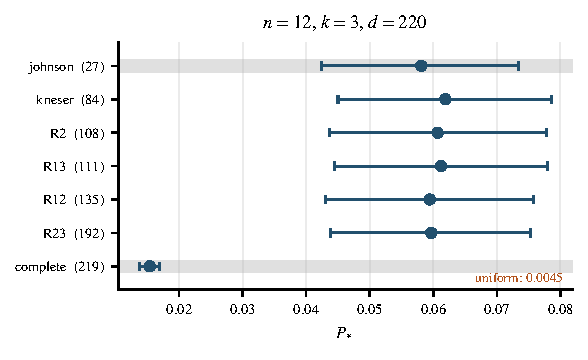
\includegraphics[width=\linewidth]{scripts/figures/fig_degree_p_opt_n12k3.pdf}
    \caption{}\label{fig:grid12a}
  \end{subfigure}\hfill
  \begin{subfigure}{0.32\textwidth}
    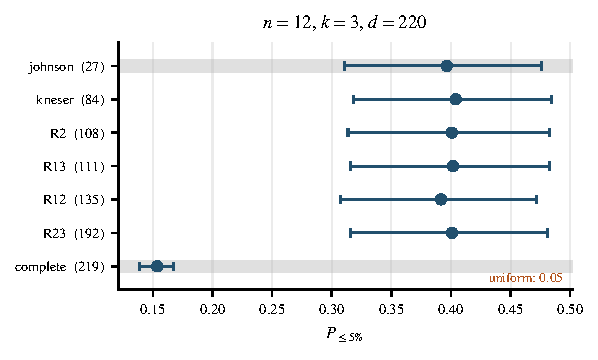
\includegraphics[width=\linewidth]{scripts/figures/fig_degree_p_top5_n12k3.pdf}
    \caption{}\label{fig:grid12b}
  \end{subfigure}\hfill
  \begin{subfigure}{0.32\textwidth}
    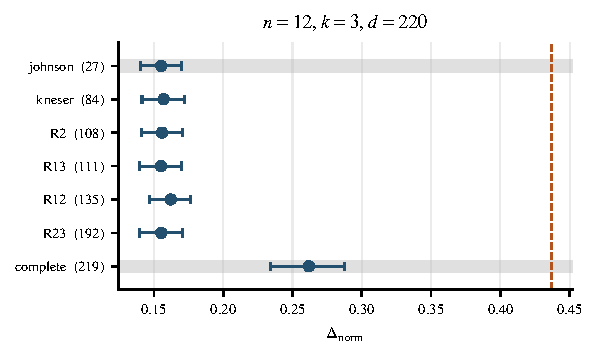
\includegraphics[width=\linewidth]{scripts/figures/fig_degree_delta_norm_n12k3.pdf}
    \caption{}\label{fig:grid12c}
  \end{subfigure}
  \caption{Single-layer performance of all seven graphs $A_T$ at
  $(n,k)=(12,3)$ over $16$ instances, ordered by degree, with the degree
  in parentheses and percentile bootstrap intervals: (a)~$P_*$,
  (b)~$P_{\le5\%}$, (c)~$\Delta_{\mathrm{norm}}$. The dashed line or
  corner annotation marks the uniform superposition; shaded rows are the
  endpoints of the family.}
  \label{fig:grid12}
\end{figure*}

\begin{figure*}[t]
  \centering
  \begin{subfigure}{0.32\textwidth}
    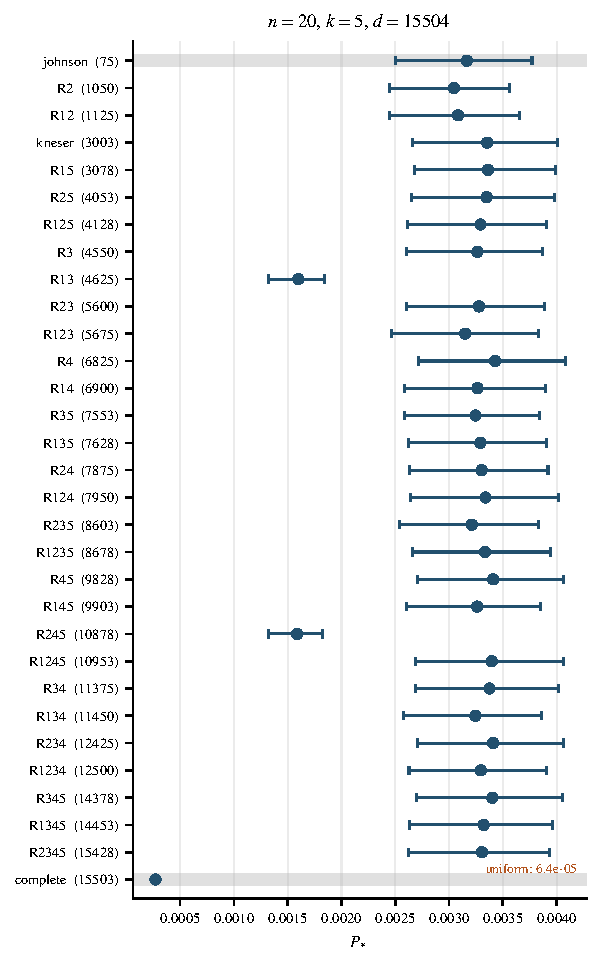
\includegraphics[width=\linewidth]{scripts/figures/fig_degree_p_opt_n20k5.pdf}
    \caption{}\label{fig:grid20a}
  \end{subfigure}\hfill
  \begin{subfigure}{0.32\textwidth}
    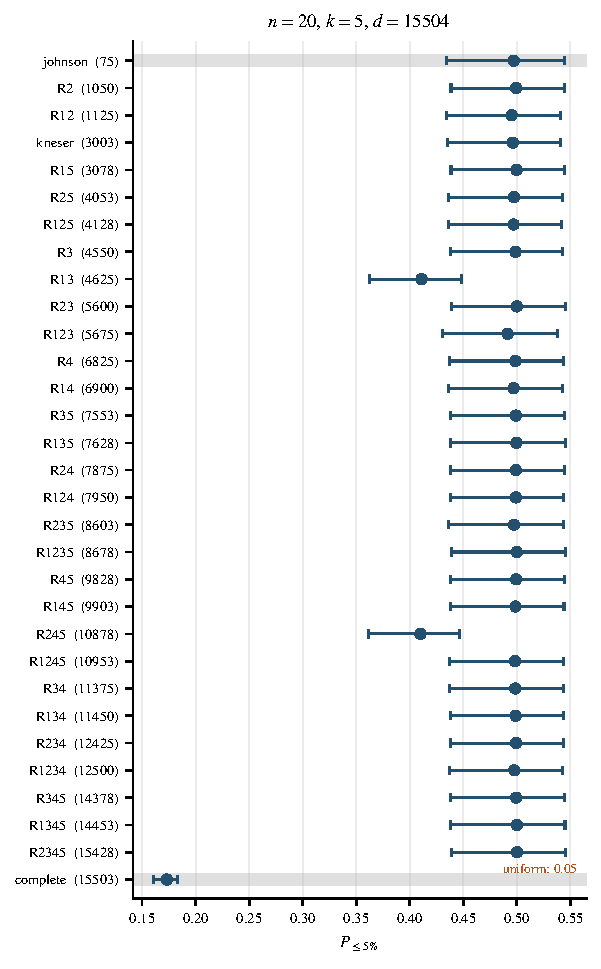
\includegraphics[width=\linewidth]{scripts/figures/fig_degree_p_top5_n20k5.pdf}
    \caption{}\label{fig:grid20b}
  \end{subfigure}\hfill
  \begin{subfigure}{0.32\textwidth}
    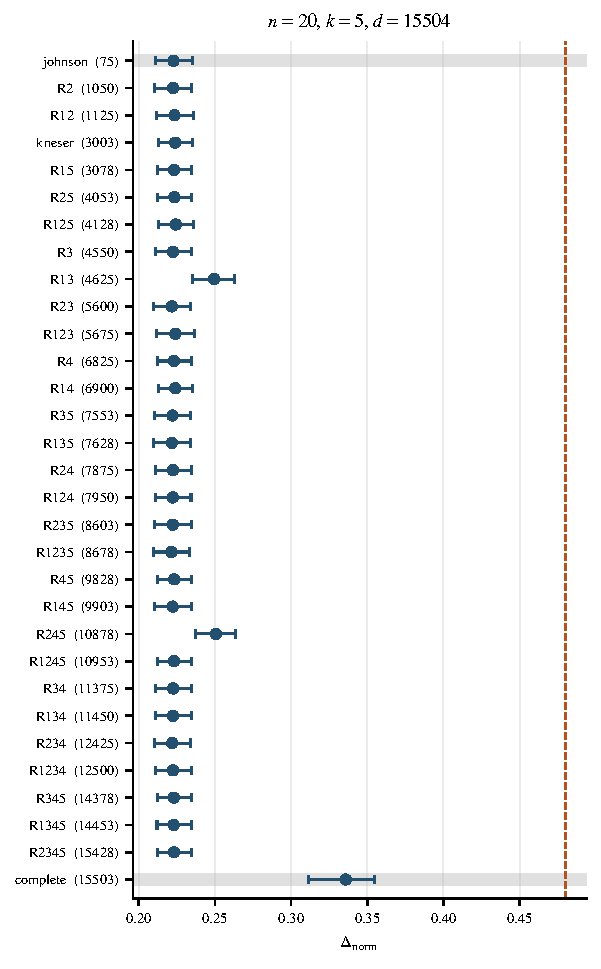
\includegraphics[width=\linewidth]{scripts/figures/fig_degree_delta_norm_n20k5.pdf}
    \caption{}\label{fig:grid20c}
  \end{subfigure}
  \caption{As Fig.~\ref{fig:grid12} for all $31$ graphs at
  $(n,k)=(20,5)$, $d=15504$, over $15$ instances, degree from $75$ to
  $15503$: (a)~$P_*$, (b)~$P_{\le5\%}$, (c)~$\Delta_{\mathrm{norm}}$.
  The two rows detached from the cluster are $R_{13}$ and $R_{245}$.}
  \label{fig:grid20}
\end{figure*}

\begin{table}[t]
  \caption{Single-layer figures of merit, mean over instances with the
  standard deviation in parentheses in units of the last digit.}
  \label{tab:grid}
  \begin{ruledtabular}
  % generated by make_tables.py
\begin{tabular}{llrccc}
$(n,k)$ & mixer & $d_{\mathrm{mix}}$ & $P_*$ & $P_{\le5\%}$ & $\Delta_{\mathrm{norm}}$ \\
\hline
(12,3) & johnson & 27 & 0.058(32) & 0.40(17) & 0.16(3) \\
 & kneser & 84 & 0.062(35) & 0.40(18) & 0.16(3) \\
 & R2 & 108 & 0.061(36) & 0.40(18) & 0.16(3) \\
 & R13 & 111 & 0.061(35) & 0.40(18) & 0.16(3) \\
 & R12 & 135 & 0.059(34) & 0.39(17) & 0.16(3) \\
 & R23 & 192 & 0.060(33) & 0.40(17) & 0.16(3) \\
 & complete & 219 & 0.015(3) & 0.15(3) & 0.26(6) \\
(16,4) & johnson & 48 & 0.013(9) & 0.41(16) & 0.18(2) \\
 & R2 & 396 & 0.012(8) & 0.39(16) & 0.19(2) \\
 & R12 & 444 & 0.011(9) & 0.35(16) & 0.22(3) \\
 & kneser & 495 & 0.014(10) & 0.40(17) & 0.19(3) \\
 & R14 & 543 & 0.013(9) & 0.40(16) & 0.18(2) \\
 & R3 & 880 & 0.014(10) & 0.41(16) & 0.18(2) \\
 & R24 & 891 & 0.0039(16) & 0.25(8) & 0.23(4) \\
 & R13 & 928 & 0.0045(18) & 0.27(9) & 0.22(4) \\
 & R124 & 939 & 0.014(10) & 0.40(16) & 0.18(2) \\
 & R23 & 1276 & 0.013(9) & 0.41(16) & 0.18(2) \\
 & R123 & 1324 & 0.014(9) & 0.41(16) & 0.18(2) \\
 & R34 & 1375 & 0.012(9) & 0.35(14) & 0.21(3) \\
 & R134 & 1423 & 0.012(8) & 0.39(15) & 0.19(3) \\
 & R234 & 1771 & 0.014(10) & 0.40(16) & 0.18(2) \\
 & complete & 1819 & 0.0020(4) & 0.15(3) & 0.28(6) \\
(20,5) & johnson & 75 & 0.0032(13) & 0.50(11) & 0.22(2) \\
 & R2 & 1050 & 0.0030(11) & 0.50(11) & 0.22(2) \\
 & R12 & 1125 & 0.0031(12) & 0.50(11) & 0.22(2) \\
 & kneser & 3003 & 0.0034(14) & 0.50(11) & 0.22(2) \\
 & R15 & 3078 & 0.0034(13) & 0.50(11) & 0.22(2) \\
 & R25 & 4053 & 0.0033(13) & 0.50(11) & 0.22(2) \\
 & R125 & 4128 & 0.0033(13) & 0.50(11) & 0.22(2) \\
 & R3 & 4550 & 0.0033(13) & 0.50(11) & 0.22(2) \\
 & R13 & 4625 & 0.0016(5) & 0.41(9) & 0.25(3) \\
 & R23 & 5600 & 0.0033(13) & 0.50(11) & 0.22(2) \\
 & R123 & 5675 & 0.0032(14) & 0.49(11) & 0.22(3) \\
 & R4 & 6825 & 0.0034(14) & 0.50(11) & 0.22(2) \\
 & R14 & 6900 & 0.0033(13) & 0.50(11) & 0.22(2) \\
 & R35 & 7553 & 0.0032(13) & 0.50(11) & 0.22(2) \\
 & R135 & 7628 & 0.0033(13) & 0.50(11) & 0.22(2) \\
 & R24 & 7875 & 0.0033(13) & 0.50(11) & 0.22(2) \\
 & R124 & 7950 & 0.0033(14) & 0.50(11) & 0.22(2) \\
 & R235 & 8603 & 0.0032(13) & 0.50(11) & 0.22(2) \\
 & R1235 & 8678 & 0.0033(13) & 0.50(11) & 0.22(2) \\
 & R45 & 9828 & 0.0034(14) & 0.50(11) & 0.22(2) \\
 & R145 & 9903 & 0.0033(13) & 0.50(11) & 0.22(2) \\
 & R245 & 10878 & 0.0016(5) & 0.41(9) & 0.25(3) \\
 & R1245 & 10953 & 0.0034(14) & 0.50(11) & 0.22(2) \\
 & R34 & 11375 & 0.0034(13) & 0.50(11) & 0.22(2) \\
 & R134 & 11450 & 0.0032(13) & 0.50(11) & 0.22(2) \\
 & R234 & 12425 & 0.0034(14) & 0.50(11) & 0.22(2) \\
 & R1234 & 12500 & 0.0033(13) & 0.50(11) & 0.22(2) \\
 & R345 & 14378 & 0.0034(14) & 0.50(11) & 0.22(2) \\
 & R1345 & 14453 & 0.0033(13) & 0.50(11) & 0.22(2) \\
 & R2345 & 15428 & 0.0033(13) & 0.50(11) & 0.22(2) \\
 & complete & 15503 & 0.00027(3) & 0.17(2) & 0.34(4) \\
\end{tabular}

  \end{ruledtabular}
\end{table}

\subsection{\label{sec:depth}Depth dependence}
At $(16,4)$, Fig.~\ref{fig:depth16}, $J(n,k)$ leads on all three metrics
at every depth and no mixer exceeds it on any instance at $p=6$, where it
reaches $P_*=0.0397$ against $0.0342$ for the Kneser graph, $0.0255$ for
$R_{23}$, $0.0190$ for $R_2$, $0.0157$ for $R_{13}$ and $0.0081$ for
$K_{\F}$; $\Delta_{\mathrm{norm}}=0.1215$ against $0.1421$ and $0.1621$
for the latter two. At $(12,3)$ $J(n,k)$ leads at $p\le3$ and is matched
or exceeded by $R_{13}$ from $p=4$ on, but $K_{\F}$ is last at every
depth there as well. Depth separates what a
single layer does not.

\begin{figure*}[t]
  \centering
  \begin{subfigure}{0.32\textwidth}
    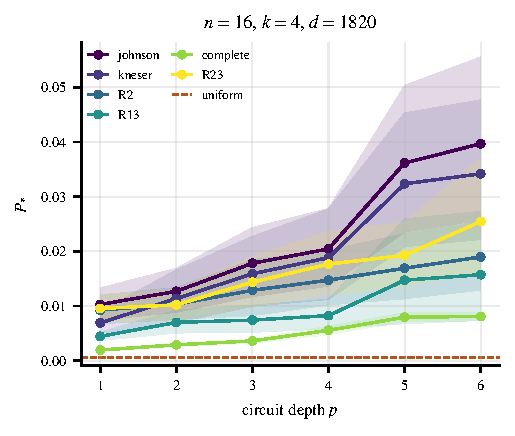
\includegraphics[width=\linewidth]{scripts/figures/fig_depth_p_opt_n16k4.pdf}
    \caption{}\label{fig:depth16a}
  \end{subfigure}\hfill
  \begin{subfigure}{0.32\textwidth}
    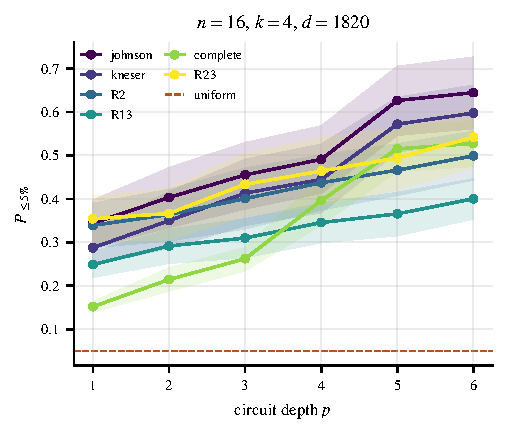
\includegraphics[width=\linewidth]{scripts/figures/fig_depth_p_top5_n16k4.pdf}
    \caption{}\label{fig:depth16b}
  \end{subfigure}\hfill
  \begin{subfigure}{0.32\textwidth}
    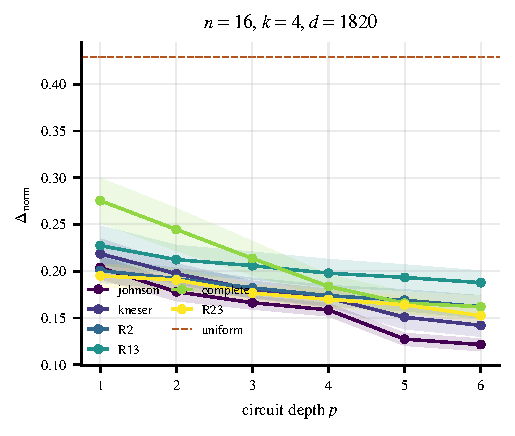
\includegraphics[width=\linewidth]{scripts/figures/fig_depth_delta_norm_n16k4.pdf}
    \caption{}\label{fig:depth16c}
  \end{subfigure}
  \caption{Performance against circuit depth at $(n,k)=(16,4)$ over $20$
  instances for six mixers spanning the degree range, layerwise
  optimisation, shaded percentile bootstrap intervals: (a)~$P_*$,
  (b)~$P_{\le5\%}$, (c)~$\Delta_{\mathrm{norm}}$.}
  \label{fig:depth16}
\end{figure*}

\begin{figure*}[t]
  \centering
  \begin{subfigure}{0.32\textwidth}
    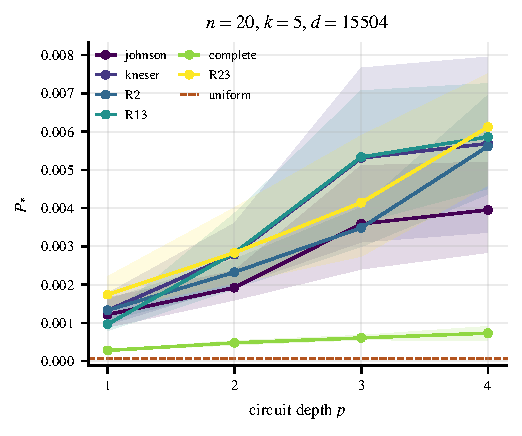
\includegraphics[width=\linewidth]{scripts/figures/fig_depth_p_opt_n20k5.pdf}
    \caption{}\label{fig:depth20a}
  \end{subfigure}\hfill
  \begin{subfigure}{0.32\textwidth}
    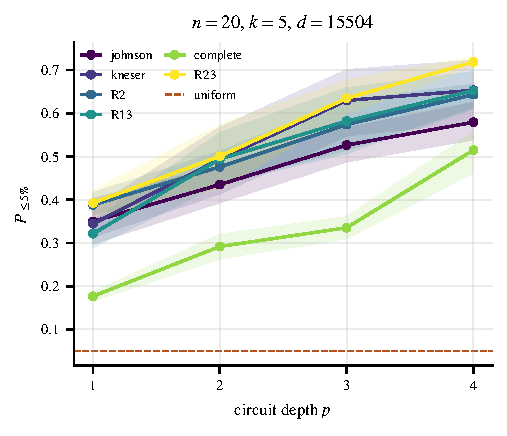
\includegraphics[width=\linewidth]{scripts/figures/fig_depth_p_top5_n20k5.pdf}
    \caption{}\label{fig:depth20b}
  \end{subfigure}\hfill
  \begin{subfigure}{0.32\textwidth}
    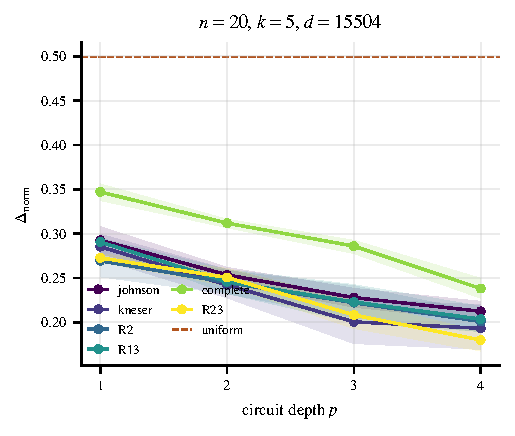
\includegraphics[width=\linewidth]{scripts/figures/fig_depth_delta_norm_n20k5.pdf}
    \caption{}\label{fig:depth20c}
  \end{subfigure}
  \caption{As Fig.~\ref{fig:depth16} at $(n,k)=(20,5)$, $d=15504$, with
  six instances and $p\le4$: (a)~$P_*$, (b)~$P_{\le5\%}$,
  (c)~$\Delta_{\mathrm{norm}}$. The ordering among the non-complete
  mixers differs from Fig.~\ref{fig:depth16}.}
  \label{fig:depth20}
\end{figure*}

\begin{table}[t]
  \caption{Optimal-sampling probability against depth, mean over
  instances with the standard deviation in parentheses in units of the
  last digit.}
  \label{tab:depth}
  \begin{ruledtabular}
  % generated by make_tables.py
% $(n,k)=(12,3)$
\begin{tabular}{lcccccc}
mixer & $p=1$ & $p=2$ & $p=3$ & $p=4$ & $p=5$ & $p=6$ \\
\hline
johnson & 0.056(30) & 0.060(32) & 0.069(39) & 0.072(40) & 0.10(6) & 0.11(6) \\
kneser & 0.041(19) & 0.044(21) & 0.061(40) & 0.064(40) & 0.080(51) & 0.092(62) \\
R2 & 0.046(21) & 0.052(29) & 0.063(28) & 0.073(44) & 0.079(42) & 0.086(45) \\
R13 & 0.040(21) & 0.046(26) & 0.049(26) & 0.096(59) & 0.100(64) & 0.11(7) \\
R12 & 0.032(13) & 0.040(20) & 0.069(49) & 0.074(51) & 0.073(46) & 0.080(49) \\
complete & 0.015(3) & 0.023(7) & 0.029(7) & 0.038(15) & 0.057(20) & 0.066(22) \\
\end{tabular}

% $(n,k)=(16,4)$
\begin{tabular}{lcccccc}
mixer & $p=1$ & $p=2$ & $p=3$ & $p=4$ & $p=5$ & $p=6$ \\
\hline
johnson & 0.010(7) & 0.013(9) & 0.018(15) & 0.020(17) & 0.036(31) & 0.040(35) \\
R2 & 0.0093(61) & 0.010(7) & 0.013(12) & 0.015(12) & 0.017(14) & 0.019(15) \\
kneser & 0.0069(48) & 0.011(11) & 0.016(15) & 0.019(19) & 0.032(29) & 0.034(30) \\
R13 & 0.0045(18) & 0.0070(49) & 0.0074(58) & 0.0083(63) & 0.015(23) & 0.016(24) \\
R23 & 0.0096(58) & 0.010(7) & 0.014(11) & 0.018(13) & 0.019(14) & 0.025(25) \\
complete & 0.0020(4) & 0.0029(8) & 0.0036(9) & 0.0056(18) & 0.0080(19) & 0.0081(19) \\
\end{tabular}

% $(n,k)=(20,5)$
\begin{tabular}{lcccc}
mixer & $p=1$ & $p=2$ & $p=3$ & $p=4$ \\
\hline
johnson & 0.0012(5) & 0.0019(5) & 0.0036(19) & 0.0040(16) \\
R2 & 0.0013(4) & 0.0023(5) & 0.0035(7) & 0.0056(18) \\
kneser & 0.0013(6) & 0.0028(11) & 0.0053(33) & 0.0057(33) \\
R13 & 0.00096(23) & 0.0028(13) & 0.0053(24) & 0.0059(19) \\
R23 & 0.0017(6) & 0.0028(14) & 0.0041(21) & 0.0061(20) \\
complete & 0.00028(2) & 0.00048(8) & 0.00061(8) & 0.00073(25) \\
\end{tabular}


  \end{ruledtabular}
\end{table}

At $(20,5)$, Fig.~\ref{fig:depth20}, the ordering inverts:

{\color{red}\textbf{[REVIEW -- overstatement from six instances]} Use ``the observed ordering differs in this six-instance subset.'' The sample is too small to establish a size-dependent inversion.} with $p\le4$
and six instances $J(n,k)$ is the weakest of the five non-complete
mixers, at $P_*=0.0040$ against $0.0061$ for $R_{23}$, $0.0059$ for
$R_{13}$, $0.0057$ for Kneser and $0.0056$ for $R_2$, and last again in
$\Delta_{\mathrm{norm}}$ at $0.2126$ against $0.1802$ for $R_{23}$, which
beats it on all six instances. Six instances are too few to establish a
reversal and the intervals overlap heavily, but too many to dismiss the
disagreement with $(16,4)$.

Note also that $R_{13}$, one of the two second-tier outliers at $(20,5)$
where it reaches half the single-layer $P_*$ of $J(n,k)$, is among the
best at $p=4$. Single-layer performance is not predictive of depth
performance within this family. What survives every size and depth is
the position of $K_{\F}$, last everywhere and by the widest margin at
$p=1$. Values are in Table~\ref{tab:depth}.

\subsection{\label{sec:circuits}Circuit realisation}
Degree on $\F_{n,k}$ is not cost on hardware; locality of the generator
is. Three regimes occur and they do not follow the degree ordering.

$A_1=J(n,k)$ is generated by the $XY$ mixer on $K_n$,
\begin{equation}
    H_{A_1}=\tfrac12\sum_{i<j}\bigl(X_iX_j+Y_iY_j\bigr),
    \label{eq:xy-mixer}
\end{equation}
two-local with $n(n-1)/2$ non-commuting terms. Terms sharing a qubit do not commute, so
$e^{-i\beta H_{A_1}}$ cannot be written as a product of the individual
exponentials and is instead approximated by a Trotter product of $r$
slices, each applying every term at angle $\beta/r$; the error falls as
$\beta^{2}/r$ and the gate count grows as $r$.

{\color{red}\textbf{[REVIEW -- Trotter precision]} Specify the exact product formula/order and the norm or observable under which this scaling is invoked, including system-size/commutator dependence.} A
proper edge colouring of $K_n$ into $n-1$ matchings schedules one step as
$n-1$ layers of disjoint two-qubit $XY$ rotations, each compiling to two
\textsc{cnot}s: $n(n-1)$ \textsc{cnot}s at depth $n-1$.

$A_j$ with $j\ge2$ exchanges $j$ assets at once, so its generator is a
sum of $\binom{n}{2j}\binom{2j}{j}/2$ hopping terms
$\prod_{a\in A}\sigma^-_a\prod_{b\in B}\sigma^+_b+\mathrm{h.c.}$, each
expanding into $2^{2j-1}$ Pauli strings of weight $2j$ needing $2(2j-1)$
\textsc{cnot}s. No union containing such a relation is two-local.

$K_{\F}$ has $A=J-I$, so
\begin{equation}
    e^{-i\beta A}=e^{i\beta}\Bigl[I
      +\bigl(e^{-i\beta|\F|}-1\bigr)\ket{s}\!\bra{s}\Bigr],
    \label{eq:grover-mixer}
\end{equation}
the Grover mixer, realised exactly as $U_S\,P\,U_S^{\dagger}$ with $U_S$
a Dicke preparation and $P$ a phase on $\ket{0}^{\otimes n}$. It carries
no Trotter error, at the price of two applications of $U_S$ and an
$n$-controlled phase. Table~\ref{tab:circuits} gives counts from explicit
construction and transpilation; entries for $j\ge2$ are lower bounds
assuming neither cancellation nor parallelism.

\begin{table}[t]
  \caption{Cost of one layer, transpiled to $\{\textsc{cnot},U\}$ with
  all-to-all connectivity. $K_{\F}$ is exact and needs one application;
  $J(n,k)$ needs $r$ Trotter steps. Entries for $j\ge2$ are lower bounds
  and no circuit was built for them.}
  \label{tab:circuits}
  \begin{ruledtabular}
  \begin{tabular}{llcrr}
    $(n,k)$ & mixer & locality & \textsc{cnot} & depth \\ \hline
    $(12,3)$ & $J(n,k)$ & 2  & 132  & 45   \\
             & $K_{\F}$ & -- & 948  & 1375 \\
             & $A_2$    & 4  & $\ge7\times10^{4}$ & -- \\[2pt]
    $(16,4)$ & $J(n,k)$ & 2  & 240  & 61   \\
             & $K_{\F}$ & -- & 1884 & 2808 \\
             & $A_2$    & 4  & $\ge3\times10^{5}$ & -- \\[2pt]
    $(20,5)$ & $J(n,k)$ & 2  & 380  & 77   \\
             & $K_{\F}$ & -- & 3124 & 4753 \\
             & $A_2$    & 4  & $\ge7\times10^{5}$ & -- \\
             & $A_3$    & 6  & $\ge1\times10^{8}$ & -- \\
  \end{tabular}
  \end{ruledtabular}
\end{table}

\subsection{\label{sec:nisq}Implications for near-term implementation}
Only $A_1$ is two-local. Unions containing $j\ge2$ need one Trotter step
of $\ge7\times10^{5}$ \textsc{cnot}s for $A_2$ and $\ge10^{8}$ for $A_3$
at $(20,5)$, against $380$ for $J(n,k)$; they map the family but are not
candidates for hardware. Of the two implementable members, $K_{\F}$ is
exact but costs $3124$ \textsc{cnot}s at depth $4753$ at $(20,5)$,
against $380$ and $77$ per Trotter step of the $XY$ mixer, so the latter
is cheaper for any Trotter order $r\lesssim8$ and by a factor of $60$ in
depth.

{\color{red}\textbf{[REVIEW -- unmatched accuracy]} This compares exact Grover evolution with approximate Johnson evolution. Quantify Trotter convergence and compare resource counts at matched error.}

{\color{red}\textbf{[LITERATURE UPDATE -- Trotter benchmark]} He et al.~\cite{He2023} already study the effect of Trotter approximation on $XY$-mixer QAOA performance, including ring/complete connectivity and noisy/hardware experiments. The manuscript should benchmark its Trotter-resource claim against that literature and avoid presenting Trotter sensitivity as an unexplored issue. A matched-error comparison remains a useful new experiment here because the present paper compares Johnson evolution with exact complete-feasible/Grover evolution.}

{\color{red}\textbf{[LITERATURE UPDATE 2026 -- XY Trotterization]} Awasthi et al.~\cite{Awasthi2026Trotter} now analyze Trotter errors for constraint-preserving $XY$ mixers and identify constraint size/locality as a key determinant; portfolio optimization is one of their benchmarks. This strengthens the need for a matched-error resource comparison and means the manuscript should not treat the $\beta^2/r$ statement as sufficient implementation evidence.}

{\color{red}\textbf{[LITERATURE UPDATE 2026 -- warm-start/topology]} Bucher et al.~\cite{Bucher2026WarmStart} construct iterative warm-start $XY$ mixers with explicit ground-state alignment and hardware validation. Together with Kordonowy and Leipold~\cite{Kordonowy2026}, this reinforces that trainability, initialization, and topology are experimentally relevant design variables and should be separated from pure feasible-graph expressivity.}

The results are favourable, the whole cluster performs within $8\%$ of itself across two
orders of magnitude in degree, so the sparsest and only two-local member
costs almost nothing in quality, and at $(16,4)$ nothing at all, leading
every tested mixer at every depth and reaching $P_*=0.0397$ at $p=6$
against $0.0081$ for $K_{\F}$.

Two further observations belong here. At $(20,5)$ and $p\le4$, $J(n,k)$ is the weakest of
the five non-complete mixers tested, so its depth advantage may not
persist with size; six instances cannot settle this. And the leaders
there, $R_{23}$ and $R_{13}$, need $\ge10^{5}$ and $\ge10^{8}$
\textsc{cnot}s per Trotter step: a factor of $1.5$ in $P_*$ at five
orders of magnitude in circuit cost is not a favourable trade at any
achievable noise level, so the practical conclusion holds where the
numerical ordering does not.

{\color{red}\textbf{[REVIEW -- unsupported noise claim]} No noise model/device data are presented. Remove ``at any achievable noise level'' or add noise-aware simulations including shots, two-qubit error, topology/routing, and ideally a device.}

$K_{\F}$ is the one unambiguous negative result:

{\color{red}\textbf{[REVIEW -- empirical scope]} Prefer ``Within the tested instances, depths, and optimization protocol, $K_{\F}$ is the most consistent negative result.''} weakest at every size
and depth, beaten by $J(n,k)$ on every instance, and the more expensive
of the two implementable mixers by factors of eight in \textsc{cnot}s and
sixty in depth, against a single Trotter step of the $XY$ mixer. Its
appeal is generality, applying to any feasible set
whose uniform superposition can be prepared and carrying no Trotter
error. Where the feasible set has combinatorial structure, discarding it
is costly in both quality and circuit resources.

{\color{red}\textbf{[REVIEW -- overgeneralization]} Restrict this to the fixed-cardinality Johnson-scheme benchmark. Resource superiority also remains unproven at matched implementation error.}

{\color{red}\textbf{[LITERATURE UPDATE -- optimizer evidence]} Scursulim et al.~\cite{Scursulim2026} compare multiple classical optimizers for a Dicke-state portfolio ansatz and report strong optimizer dependence, with CMA-ES performing particularly well in their experiments. This does not establish that CMA-ES is optimal for the present QWOA landscape, but it provides a directly relevant portfolio/Dicke precedent for an optimizer ablation against COBYLA.}
